\chapter{Arrays of Objects}

\begin{exercise}
Consider this UML diagram for a \java{City} class in Figure~\ref{fig.cityuml}

\begin{figure}[!h]
\begin{center}
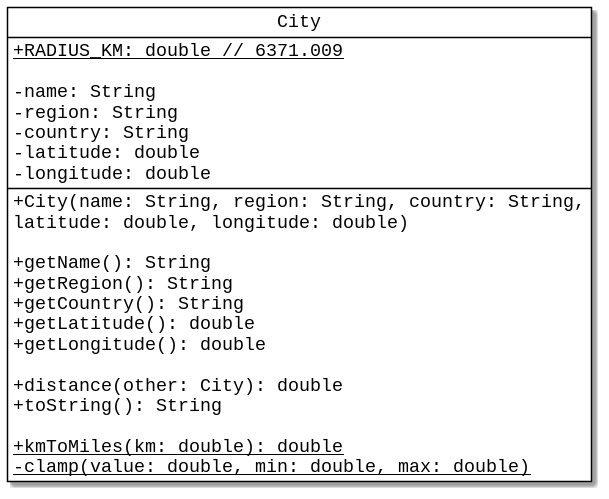
\includegraphics[scale=0.5]{figs/ch12/city.png}
\caption{UML Diagram for a City class}
\label{fig.cityuml}
\end{center}
\end{figure}

The class has private instance variables for the city name, its region (for the US, it's called a state; for Canada, it's a province; for Japan it's a prefecture), and its latitude and longitude measured in degrees.

This is an immutable class. (How would you determine this from the UML diagram?)

\java{RADIUS_KM} is a \java{static} \java{final} constant representing the radius of the earth in kilometers.

The constructor will make sure that the longitude is in the range -180 to 180 and the latitude in the range -90 to 90. The constructor will use the \java{clamp} method to enforce this:

\begin{code}
private static double clamp(double value, double min, double max) {
    double result = value;
    if (value <  min) {
        result = min;
    }
    else if (value > max) {
        result = max;
    }
    return result;
}
\end{code}


Question: why do you think this method was declared \java{private} instead of \java{public}? Why is it a \java{static} method instead of an instance method?

The \java{distance} method will calculate the great circle distance between one \java{City} object and the \java{other} \java{City} object. Here is the formula where $r$ is the radius of earth in kilometers (6371.009), the first city's latitude and longitude are $lat_1$, $lon_1$ and the second city's latitude and longitude are  $lat_2$, $lon_2$:

\begin{equation*}
d = r\cdot cos^{-1}(sin(lat_1)\cdot sin(lat_2) + cos(lat_1)\cdot cos(lat_2)\cdot cos(lon_1 - lon_2))
\end{equation*}


\end{exercise}
